\section{Overview}

\begin{figure*}[h]
    \centering
      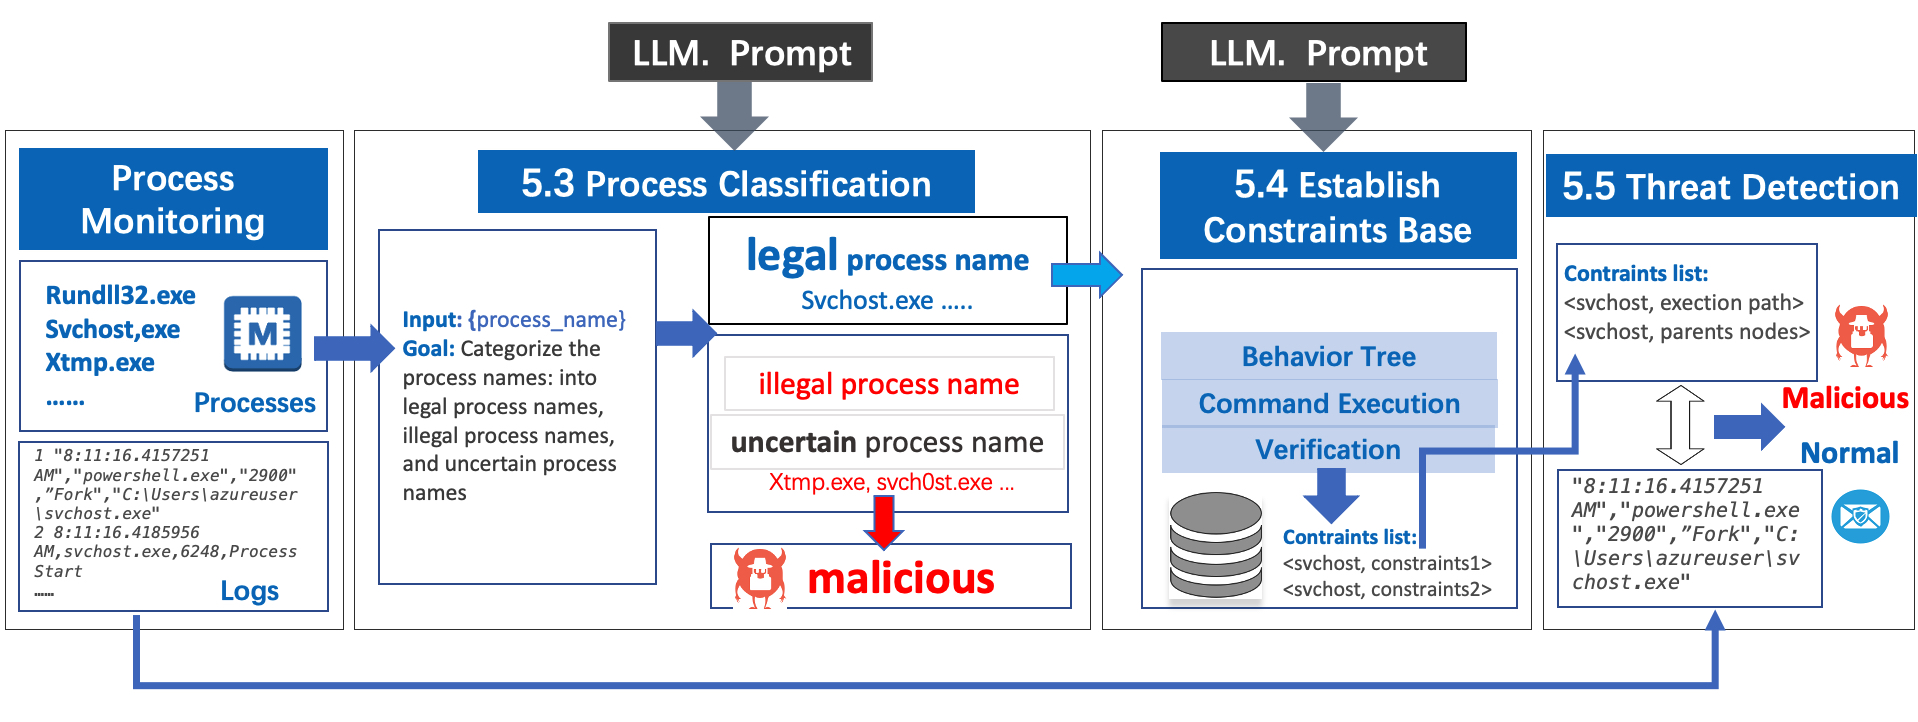
\includegraphics[width=1\textwidth]{figs/framework.jpg}
    \caption{We collect system process logs and, with the aid of LLM, categorize them into: legitimate, illegitimate, and uncertain process names. Processes labeled as uncertain or illegitimate are flagged for security analyst review (detailed in Section 5.3). For those deemed legitimate, LLM assists in constructing a process constraint database. This is achieved through behavior tree creation, command execution, and validation (explained in Section 5.4). Logs that violate these constraints are indicative of potential threats (detailed in Section 5.5).}
    \label{fig-framework}
    \end{figure*}

\subsection{Threat Model}
In this paper, we focus on detecting and tracing anomalous entities in a host caused by intrusion campaigns. We assume the adversary has the following characteristics:

\begin{itemize}
    \item \textbf{Stealthy}. Instead of simply performing an attack, the attacker consciously hides their malicious activities, trying to mix their behavior with a large amount of benign background data, which makes the victim system perform like a benign mode.
    \item \textbf{Persistent}. These adversaries don't just execute short-lived attacks. Instead, they maintain a prolonged presence within systems, continuously adapting their attack strategies to circumvent emerging defense measures.
    \item \textbf{Frequent usage of zero-day exploits}. The attacker tends to use zero-day exploits to attack a system. Therefore, we assume that we do not have any attack patterns for training.
\end{itemize}


Our proposed system revolves around the hypothesis that the observation of ubiquitous OS kernel processes is a feasible alternative to sample-focused analysis. Unlike suspicious samples, system processes are present at all times and do not need to be identified prior to analysis.

\subsection{Overview}
As illustrated in Figure~\ref{fig-framework}, we utilized a log collection tool to gather logs from various system processes. Harnessing the formidable capabilities of LLM, we categorized these processes based on their names into three distinct classes: legitimate process names, illegitimate process names, and uncertain process names (owing to the inherent incompleteness of the GPT's database). For the latter two categories, we marked them as potentially malicious, warranting further investigation by security analysts. A more in-depth examination of this process is provided in Section 5.3.

For processes classified with legitimate names, we employed the LLM to construct a database delineating normal process constraints. This primarily encompasses three stages: developing the process behavior tree, executing commands, and subsequent validation. Upon culmination, this facilitates the creation of a behavior constraint database for each process. A detailed discussion on this topic is set out in Section 5.4. Leveraging this process behavior database, we compared extracted log information against the established constraints. Any violation of these constraints is indicative of potential malicious activity.




